\section{Geometry description file}
\label{sect: annexe 1}
{\huge TO BE TRANSLATED}\\
\noindent
Ce fichier décrit la géométrie utilisée~: le nombre et le nom des surfaces maillées séparant les différents domaines de
conductivité ainsi que le nombre et le nom de chacun de ces domaines et leur disposition par rapport aux surfaces précédemment
citées.\\ 
Extension du fichier~: *.geom par convention. 

\centerline{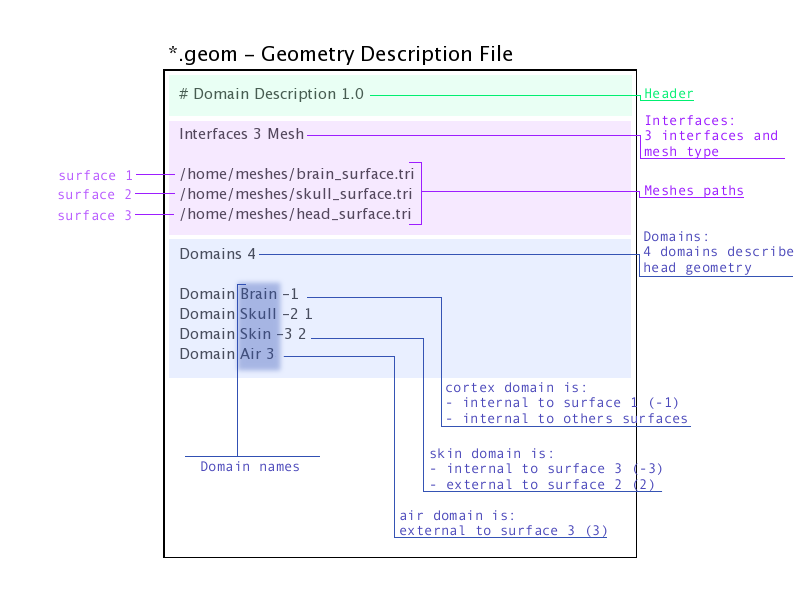
\includegraphics[height=9cm]{geom.png}}

\begin{note}
    nous avons un bug qui peut survenir sur l'ordre des domaines. Il est alors préférable de noter les domaines de la manière
    suivante (noter en premier la référence aux surfaces externes et en deuxième position la surface interne)~:

    \begin{tabular}{ll}
        Domain Brain -1              & \\
        Domain Skull \textbf{1 -2}	 &	\emph{au lieu de Domain Skull -2 1} \\
        Domain Skin \textbf{2 -3}	 &	\emph{au lieu de Domain Skin -3 2}  \\
        Domain Air 3                 &  \\
    \end{tabular}
\end{note}

\medskip

\begin{note}
    les "Meshes paths" sont 
    \begin{itemize}
        \item soit absolus (comme le montre le dessin)
        \item soit relatifs à l'endroit où on exécute les lignes de commandes 
    \end{itemize}
    Seuls les formats suivants sont lus pour les surfaces maillées~:
    \begin{itemize}
        \item *.tri~: format TRI issu des premières versions de BrainVisa. Aussi lu par Anatomist.
        \item *.mesh~: format MESH issu des versions 3.0.2 et plus de BrainVisa. Aussi lu par Anatomist.
        \item *.vtk~: format de maillage VTK.
    \end{itemize}
\end{note}


\section{Fichier de description des conductivités}
\label{sect: annexe 2}

\noindent
Ce fichier décrit les valeurs des conductivités associées aux différents domaines déclarés dans le fichier de description de la
géométrie.\\ 
Extension du fichier~: *.cond par convention.\\
\warning{Attention~:  bien respecter la casse entre les noms de domaines donnés dans le fichier de description de la géométrie et ceux
notés dans le fichier de description des conductivités !}

\centerline{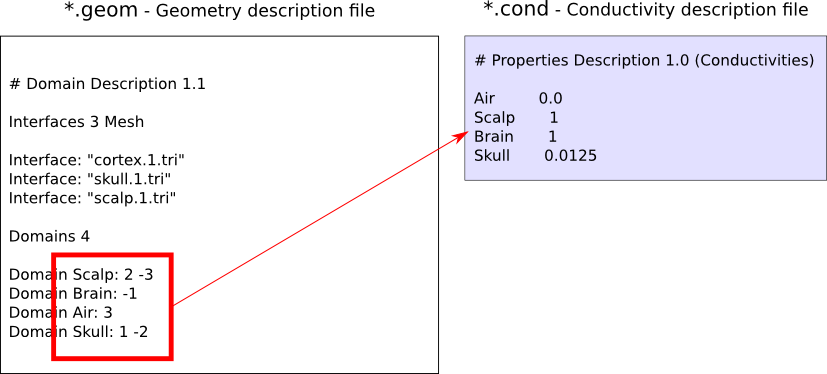
\includegraphics[height=9cm]{cond.png}}

\begin{note}
    ce sont des conductivités relatives~: l'air n'est pas conducteur, donc a une conductivité nulle, le cerveau est considéré
    comme étant entièrement conducteur tout comme la peau et le crâne a une conductivité égale à 1/80 de celle du cerveau.
\end{note}

\section{Position et orientation des dipôles}
\label{sect: annexe 3}

\noindent
Fichier texte. A une ligne donnée correspond un dipôle~: 
\begin{itemize}
    \item les trois premiers nombres (séparés par un espace) sont les coordonnées cartésiennes de la position du dipôle,
    \item les trois derniers nombres (séparés par un espace) sont les coordonnées cartésiennes du vecteur normale donnant
           l'orientation du dipôle.
\end{itemize}
Extension de fichier~: *.dip ou *.txt.

\medskip

\noindent
Dans l'exemple ci dessous, sont décrits 5 dipôles~:

\centerline{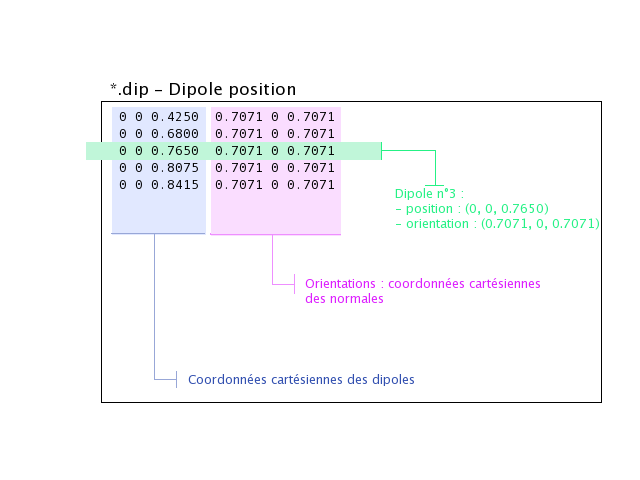
\includegraphics[height=9cm]{dipolePositions.png}}

\begin{note}
    les coordonnées sont prises dans le même repère que celui des maillages (repère de l'IRM en général)
\end{note}

\section{Position (et orientation) des capteurs}
\label{sect: annexe 4}

\noindent
Dans le cas de l'EEG, il s'agit d'un fichier de description de la position des capteurs en coordonnées cartésiennes et dans le
même repère que celui des maillages (en général, le repère de l'IRM). A une ligne correspond les coordonnées d'un capteur
séparées par un espace. 

\medskip

\noindent
Dans le cas de la MEG, il s'agit d'un fichier de description de la position et de l'orientation des capteurs en coordonnées
cartésiennes et dans le même repère que celui des maillages (en général, le repère de l'IRM). A une ligne correspond les
coordonnées d'un capteur (séparées par un espace) suivies des coordonnées du vecteur orientation normé (séparés par un espace).

\section{Activation des sources}
\label{sect: annexe 5}

\noindent
Les fichiers d'activation des sources sont des fichiers texte. A une ligne correspond une source~: 
\begin{itemize}
    \item dans le cas dipolaire, sont écrits sur la ième ligne les états d'activation du ième dipôle,
    \item dans le cas des sources distribuées, sont écrits sur la ième ligne les états d'activation du ième point du maillage
          des sources.
\end{itemize}

\medskip

\noindent
On trouve en colonne les temps auxquels sont associés les activations.

\medskip

\noindent
Exemple dans le cas dipolaire~:

\centerline{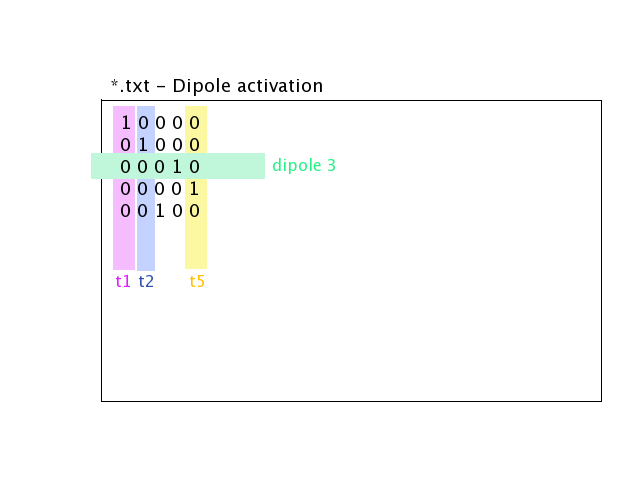
\includegraphics[height=9cm]{dipActiv.png}}
